\chapter{Подготовка к работе и порядок действий}\label{ch:preparation-ru}

\section{Подготовка автомобиля}
При замене штатной приборной панели на Digifiz соблюдайте следующую последовательность:
\begin{enumerate}
    \item Снимите пластиковые накладки над педалями и нижнюю часть панели, чтобы получить доступ к штатному щитку.
    \item Отсоедините аккумулятор автомобиля.
    \item Отсоедините жгут от заводской приборной панели.
    \item Открутите механический привод спидометра, если он установлен.
    \item Выкрутите крепёжные винты и аккуратно извлеките щиток из автомобиля.
    \item Проложите комплектные жгуты датчиков температуры и скорости согласно инструкции.
    \item Установите приборку Digifiz в направляющие кронштейна и закрепите винтами.
    \item Для \ReplicaNextLong{} установите датчики Volkswagen MFA (или эквивалентные) и протяните их провода к разъёмам CE~1/CE~2.
    \item На моделях \texttt{GACS}/\texttt{GARS}/\texttt{DARS}/\texttt{DACS} вручную подключите промаркированные провода \texttt{MFA\_MODE}, \texttt{MFA\_RESET}, \texttt{MFA\_BLOCK} и ручника, если в жгуте автомобиля нет этих контактов. Во втором поколении \ReplicaNextShort{} эти сигналы по умолчанию коммутируются внутри щитка.
    \item Подключите жгуты к приборной панели.
    \item Установите электронный датчик скорости или снова присоедините тросовый привод.
    \item Соберите облицовку панели и кожух педалей в обратном порядке.
\end{enumerate}

\section{Эксплуатация приборной панели}
\begin{itemize}
    \item Панель автоматически включается вместе с зажиганием. Подсветка управляется переключателем габаритных огней.
    \item При запуске загорается вся шкала скорости, пока внутренние диагностики стабилизируют модель оборотов; затем индикация переходит на текущие холостые.
    \item После начала движения система отображает параметры, перечисленные в \Cref{ch:technical-specs-ru}.
\end{itemize}

\subsection{Функции MFA}
Доступно шесть страниц MFA:
\begin{enumerate}
    \item Суточное время работы.
    \item Пробег поездки.
    \item Расход топлива (не реализован в первой версии Replica).
    \item Средняя скорость (значение отображается, умноженное на десять).
    \item Температура масла (требуется внешний жгут).
    \item Наружная температура (требуется внешний жгут).
\end{enumerate}
На \ReplicaGenOneShort{} переключение страниц осуществляется ёмкостной кнопкой за логотипом VW; \ReplicaNextShort{} использует внешний подрулевой переключатель.
Длительность касания влияет следующим образом:
\begin{itemize}
    \item Короткое нажатие (\(<1\)~с): переход к следующей функции MFA.
    \item Среднее нажатие (1--3~с при отсутствии подрулевого переключателя): переключение между блоками памяти MFA; изменение отображается на экране.
    \item Долгое нажатие (3--7~с): сброс активной функции MFA (влияет на расход, пробег, время и среднюю скорость).
\end{itemize}

\subsection{Подсветка и индикация}
На \ReplicaGenOneShort{} доступна ручная регулировка яркости над переключателем габаритов; \ReplicaNextShort{} использует автоматическое регулирование по фотодиоду.
Ручные режимы можно задать через сервисные интерфейсы, описанные в \Cref{ch:replica-setup-ru,ch:replica-next-setup-ru}.

Схема горизонтального блока индикаторов и пояснения к нему показаны на \autoref{fig:indicator-layout-ru}.

\begin{figure}[htbp]
    \centering
    \begin{subfigure}{0.48\textwidth}
        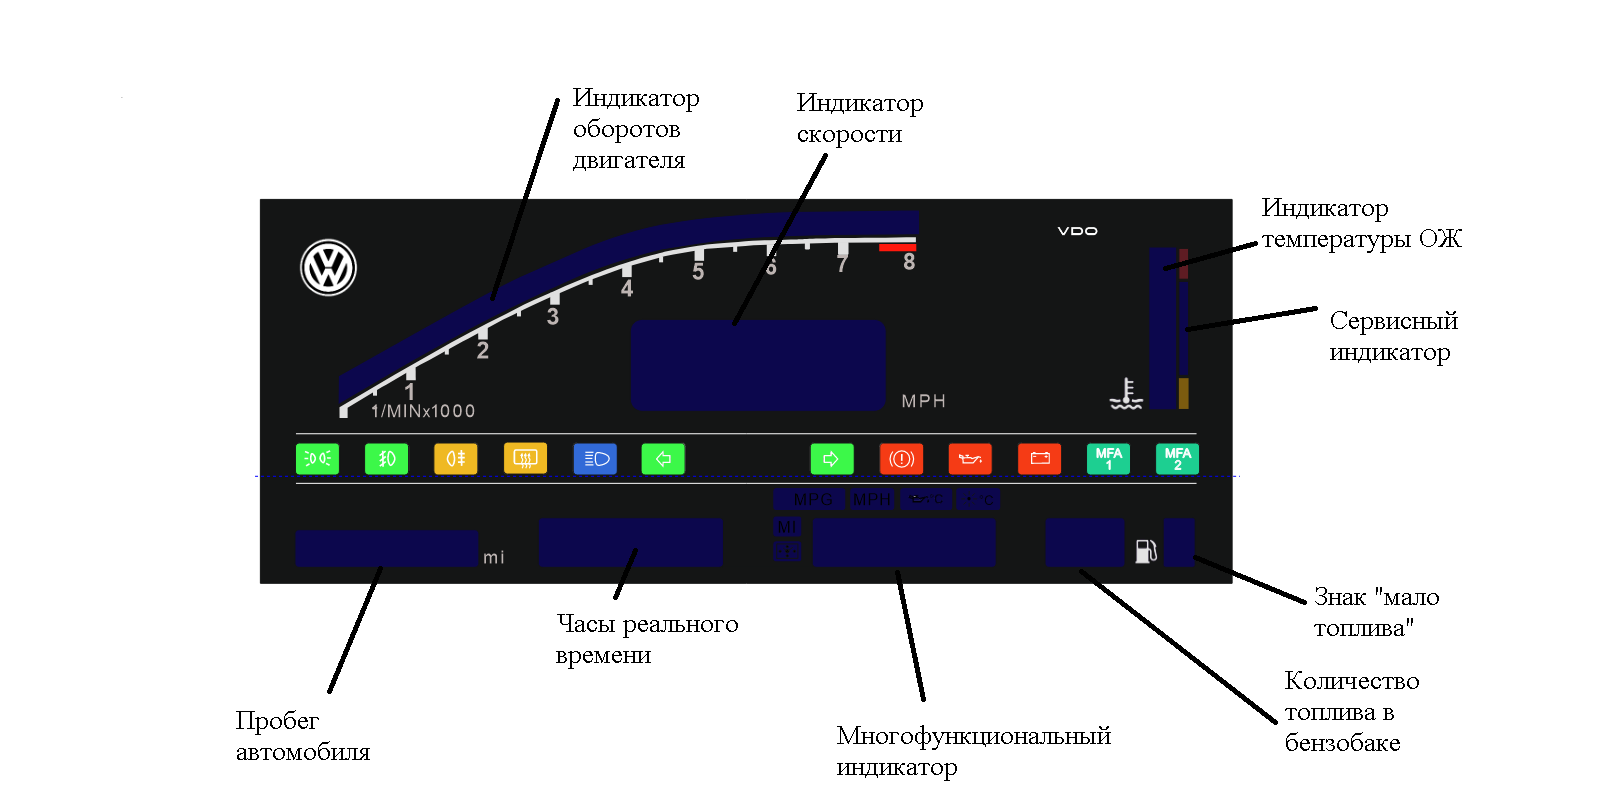
\includegraphics[width=\linewidth]{digifiz_manual/image017.png}
        \caption{Индикация в ходе самотестирования при включении.}
    \end{subfigure}\hfill
    \begin{subfigure}{0.48\textwidth}
        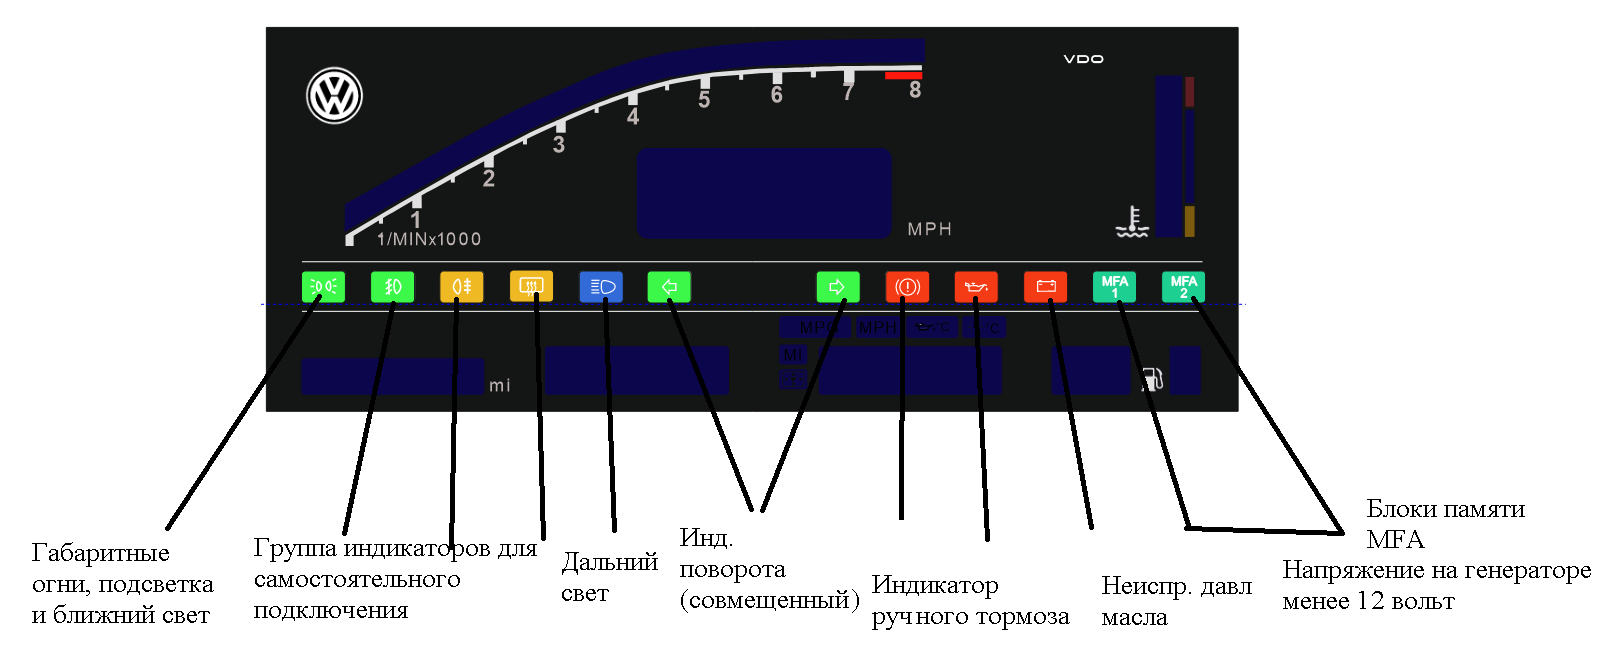
\includegraphics[width=\linewidth]{digifiz_manual/image018.png}
        \caption{Легенда горизонтальной группы индикаторов.}
    \end{subfigure}
    \caption{Схема индикации приборной панели.}
    \label{fig:indicator-layout-ru}
\end{figure}

\subsection{Интерфейсы конфигурации}
\begin{itemize}
    \item Классические блоки \ReplicaGenOne{} оснащены модулем Bluetooth 2.0 (совместимым с BLE). Установите приложение \emph{Serial Bluetooth Terminal} из Google Play, выполните спаривание с приборкой и подавайте команды из терминала. Устройства Apple iOS не поддерживают подключение к этому модулю.
    \item \ReplicaNextShort{} разворачивает встроенную Wi-Fi-точку доступа и веб-портал конфигурации, описанный в \Cref{ch:replica-next-setup-ru}. При подключении отключите мобильные данные, чтобы корректно открылась каптив-портал страница.
\end{itemize}
Обе генерации можно питать и настраивать на стенде через программатор USBasp.
